% 1977 年福建卷理科第 1(10) 题：V 形铁块示意图
% 源卷只要求据图画三视图，未给尺寸；此处重绘结构关系，不虚构尺寸。
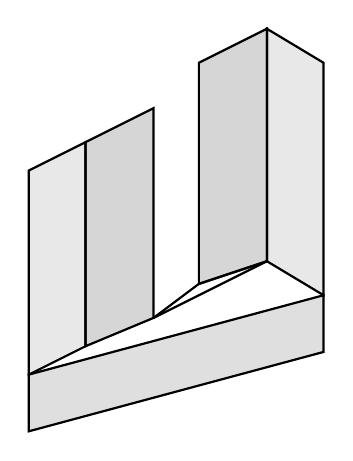
\begin{tikzpicture}[scale=0.72]
  \fill[gray!25] (0,0)--(5.2,1.4)--(5.2,2.4)--(0,1.0)--cycle;
  \draw[thick] (0,0)--(5.2,1.4)--(5.2,2.4)--(0,1.0)--cycle;
  \fill[gray!18] (0,1.0)--(0,4.6)--(1.0,5.1)--(1.0,1.5)--cycle;
  \fill[gray!32] (1.0,1.5)--(1.0,5.1)--(2.2,5.7)--(2.2,2.0)--cycle;
  \draw[thick] (0,1.0)--(0,4.6)--(1.0,5.1)--(1.0,1.5)--cycle;
  \draw[thick] (1.0,1.5)--(1.0,5.1)--(2.2,5.7)--(2.2,2.0)--cycle;
  \fill[gray!18] (5.2,2.4)--(5.2,6.5)--(4.2,7.1)--(4.2,3.0)--cycle;
  \fill[gray!32] (4.2,3.0)--(4.2,7.1)--(3.0,6.5)--(3.0,2.6)--cycle;
  \draw[thick] (5.2,2.4)--(5.2,6.5)--(4.2,7.1)--(4.2,3.0)--cycle;
  \draw[thick] (4.2,3.0)--(4.2,7.1)--(3.0,6.5)--(3.0,2.6)--cycle;
  \draw[thick] (2.2,2.0)--(3.0,2.6);
  \draw[thick] (2.2,2.0)--(4.2,3.0);
  \draw[thick] (3.0,2.6)--(4.2,3.0);
  \draw[dashed] (2.2,2.0)--(2.2,5.7);
  \draw[dashed] (3.0,2.6)--(3.0,6.5);
\end{tikzpicture}
